\subsection{Experimental Setup}

All models share the same architecture and training procedure described in
Section~\ref{sec:method}; they differ only in their training objective.
We compare four training strategies:

\begin{itemize}
    \item \textbf{L2 (MSE)} — trained with mean squared error.
    \item \textbf{L1 (MAE)} — trained with mean absolute error.
    \item \textbf{Pinball} — trained with the standard (linear) pinball loss.
    \item \textbf{PLF} — trained end-to-end with the piecewise linear asymmetric
          cost function (Section~\ref{sec:modeling}).
\end{itemize}

To isolate the benefit of end-to-end cost-aware training, we additionally
evaluate \emph{post-hoc calibrated} variants of all four models
(Section~\ref{sec:posthoc}), in which an affine transformation
$g(z)=\alpha z + \beta$ is fitted on the training set to minimise the
expected asymmetric cost.

Models are evaluated on four cost functions that reflect different assumptions
about the cost of over- and under-prediction: the piecewise linear cost
(\textbf{PLF}), the L1 cost, the L2 cost, and the standard pinball loss.
The primary metric is the \textbf{PLF} cost, which best reflects the
asymmetric, non-linear structure of real-world electricity procurement costs.

\subsection{Evaluation Cost Functions}

Figure~\ref{fig:loss_fns} illustrates the four cost functions used for
evaluation.
The PLF and pinball functions penalise under-predictions more heavily than
over-predictions, reflecting the real-world asymmetry of electricity
procurement costs, while L1 and L2 serve as symmetric reference points.

\begin{figure}[H]
    \centering
    
\includegraphics[width=\linewidth]{plot/loss_fns.png}
    \caption{The four cost functions used for evaluation: the piecewise linear
             asymmetric cost (\textbf{PLF}), the pinball loss, L1 (MAE),
             and L2 (MSE).  The PLF and pinball functions penalise
             under-predictions more heavily than over-predictions.}
    \label{fig:loss_fns}
\end{figure}

\subsection{Results}

Table~\ref{tab:eval} reports the average test-set cost of each model under
each evaluation cost function, before and after post-hoc calibration.

\begin{table}[ht]
    \centering
    \caption{Test-set cost under four evaluation metrics.  Lower is better.
             Bold marks the best value in each column.
             \emph{Top block:} raw predictions; \emph{bottom block:}
             after post-hoc affine calibration.}
    \label{tab:eval}
    \begin{tabular}{lrrrr}
        \toprule
        \textbf{Model} & \textbf{PLF} & \textbf{L1} & \textbf{L2} & \textbf{Pinball} \\
        \midrule
        \multicolumn{5}{l}{\textit{Without post-hoc calibration}} \\
        \midrule
        PLF        & \textbf{0.386} & 0.620          & 0.734          & 0.434 \\
        L1 (MAE)   & 0.407          & \textbf{0.570} & 0.647          & 0.539 \\
        L2 (MSE)   & 0.428          & 0.577          & \textbf{0.629} & 0.609 \\
        Pinball    & 0.438          & 0.802          & 1.084          & \textbf{0.370} \\
        \midrule
        \multicolumn{5}{l}{\textit{With post-hoc affine calibration}} \\
        \midrule
        PLF + calibration     & \textbf{0.386} & 0.577          & 0.654          & 0.373 \\
        L1 + calibration      & 0.396          & 0.570          & 0.643          & 0.382 \\
        L2 + calibration      & 0.388          & \textbf{0.569} & \textbf{0.629} & 0.377 \\
        Pinball + calibration & 1.309          & 0.584          & 0.753          & \textbf{0.370} \\
        \bottomrule
    \end{tabular}
\end{table}

Figure~\ref{fig:confusion-matrix} visualises the same results as a colour-coded
model~$\times$~loss matrix, making it easy to see at a glance which model wins
on each metric and how calibration shifts the ranking.

\begin{figure}[H]
    \centering
    
\includegraphics[width=\linewidth]{plot/confusion_matrix.png}
    \caption{Train-loss~$\times$~evaluation-metric matrix for the three models
             (L1, Pinball~5:1, Pinball~20:1), before calibration (left) and
             after post-hoc affine calibration (right).  Each cell shows the
             test-set cost; green marks the best value in each column and red
             the worst.  The diagonal tendency --- each model achieving its
             lowest cost on the metric it was trained with --- is clearly
             visible.  Calibration reduces off-diagonal costs substantially
             (e.g.\ L1 model under Pinball~20:1 drops from 3.167 to 1.022)
             while leaving the diagonal unchanged.}
    \label{fig:confusion-matrix}
\end{figure}

\subsection{Discussion}

\paragraph{Each model excels on its own training metric.}
Without calibration, a clear diagonal dominance is visible in
Figure~\ref{fig:confusion-matrix}: each model achieves its lowest cost on
the metric it was trained to minimise.
The L1 model produces the lowest L1 cost ($2.704$), the Pinball~5:1 model
the lowest Pinball~5:1 cost ($1.820$), and the Pinball~20:1 model the lowest
Pinball~20:1 cost ($0.841$).
This confirms that the training objective directly shapes the cost profile
of the resulting forecast.

\paragraph{Asymmetric training substantially outperforms the symmetric baseline.}
The advantage of cost-aware training grows with the asymmetry ratio.
Under the Pinball~5:1 metric, the Pinball~5:1 model ($1.820$) outperforms
the L1 baseline ($3.045$) by $40\%$.
Under the more demanding Pinball~20:1 metric, the Pinball~20:1 model
($0.841$) outperforms L1 ($3.167$) by $73\%$.
Figure~\ref{fig:error_histograms} shows the mechanism: the Pinball~20:1
model produces a heavily right-skewed error distribution, deliberately
over-predicting to avoid costly under-procurement events, while the L1
model is symmetric and centred near zero.

\paragraph{Post-hoc calibration narrows but does not close the gap.}
Affine calibration substantially improves the L1 model on asymmetric metrics
(Pinball~20:1: $3.167 \to 1.022$; Pinball~5:1: $3.045 \to 1.979$),
confirming that a global bias correction captures much of the asymmetric
signal.
However, calibrated L1 still falls short of the dedicated pinball models
(Pinball~5:1: $0.851$; Pinball~20:1: $0.841$), because a single affine
shift cannot replicate the input-conditional upward bias that end-to-end
cost-aware training achieves.
Figure~\ref{fig:error-heatmap} (Section~\ref{sec:forecast-error-dist})
illustrates exactly why: forecast error magnitude varies substantially by
hour of the day and day of the week.
A uniform global correction applies the same rescaling to every prediction
regardless of context; only a model that conditions its output on time
features can adapt its bias to each slot individually.

\paragraph{Error distributions reflect the targeted quantile.}
Figure~\ref{fig:error_histograms} shows the prediction error distributions
on the test set for each model.
The L1 model is symmetric and centred near zero, as expected for a
mean-unbiased estimator.
The Pinball~5:1 model is modestly right-shifted, and the Pinball~20:1 model
exhibits a pronounced positive tail --- each distribution directly reflecting
the quantile targeted by its respective asymmetric loss.

\begin{figure}[H]
    \centering
    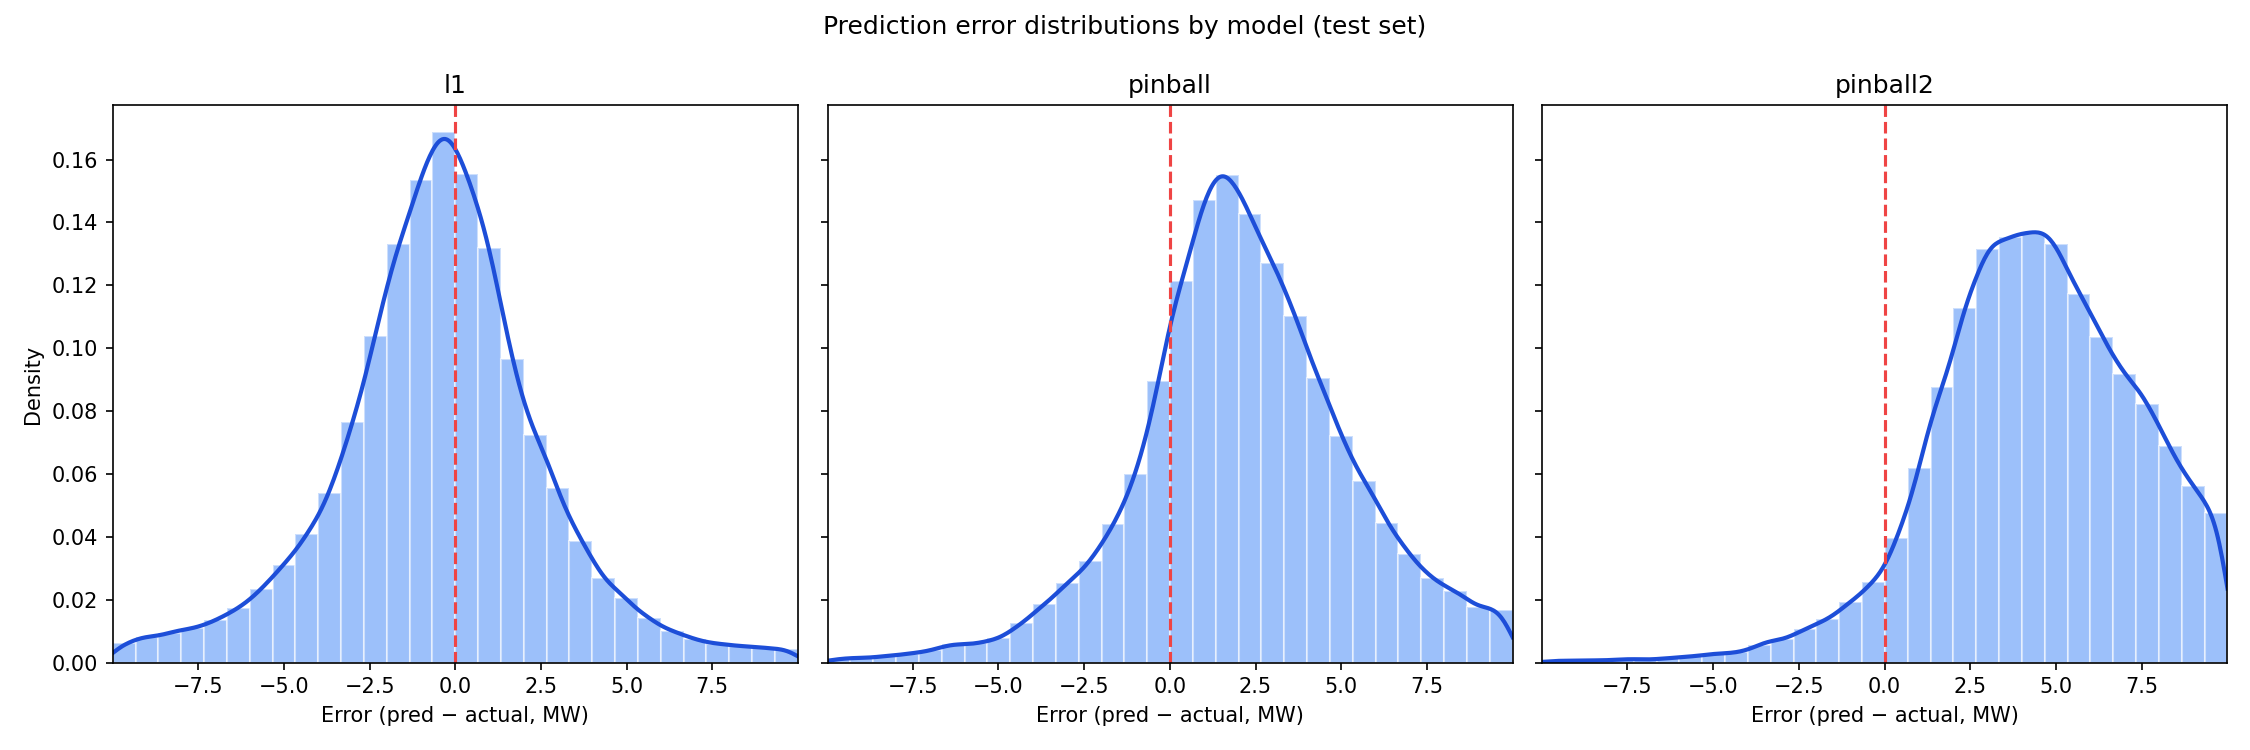
\includegraphics[width=\linewidth]{plot/error_histograms.png}
    \caption{Distribution of test-set prediction errors (forecast minus
             actual, MW) for each model.  The L1 model is symmetric and
             centred near zero.  The Pinball~5:1 model shows a modest
             rightward shift, and the Pinball~20:1 model a pronounced
             positive tail, reflecting the increasingly aggressive upward
             bias required to minimise the cost under higher asymmetry ratios.}
    \label{fig:error_histograms}
\end{figure}

